\documentclass[12pt,a4paper]{article}

\usepackage[utf8]{vietnam}
\usepackage[vietnamese=nohyphenation]{hyphsubst}
\usepackage[vietnamese]{babel}
\usepackage[T1]{fontenc}
\usepackage{lmodern}
\usepackage{amsmath,amssymb}
\usepackage{graphicx}
\usepackage{booktabs}
\usepackage{tabularx}
\usepackage{array}
\usepackage{enumitem}
\usepackage{setspace}
\usepackage{xcolor}
\usepackage{float}
\usepackage{caption}
\usepackage{fancyhdr}
\usepackage{titlesec}
\usepackage[
  margin=2.2cm,
  top=2.4cm,
  bottom=2.4cm,
  headheight=14pt
]{geometry}
\usepackage{hyperref}
\DeclareUrlCommand\code{\urlstyle{tt}}
\setlength{\emergencystretch}{3em}

\hypersetup{
  colorlinks=true,
  linkcolor=black,
  urlcolor=blue!50!black,
  citecolor=black
}

\pagestyle{fancy}
\fancyhf{}
\fancyhead[L]{\small Topic Team --- DLinear \& NLinear}
\fancyhead[R]{\small WEEK02 STL Reading Note}
\fancyfoot[C]{\thepage}
\renewcommand{\headrulewidth}{0.4pt}

\titleformat{\section}{\large\bfseries}{\thesection.}{0.6em}{}
\titleformat{\subsection}{\normalsize\bfseries}{\thesubsection.}{0.5em}{}
\setlist[itemize]{leftmargin=1.4em, itemsep=0.25em, topsep=0.35em}
\onehalfspacing

% Cornell: Cue | Detail
\newcolumntype{C}{>{\raggedright\arraybackslash}p{0.26\textwidth}}
\newcolumntype{D}{>{\raggedright\arraybackslash}X}
\newcommand{\cornellhead}{%
  \toprule
  \textbf{Cue / Question} & \textbf{Detail} \\
  \midrule
}

\begin{document}

\begin{center}
  {\LARGE\bfseries Ghi chép đọc --- STL \& Loess}\\[0.35em]
  {\large Seasonal-Trend decomposition using Loess}\\[0.5em]
  {\normalsize Topic Team AIO2026 --- So sánh DLinear \& NLinear}\\[0.25em]
  {\small WEEK02 Reading Note --- Cornell (bảng); scan tay ở Phụ lục}
\end{center}

\vspace{0.5em}
\noindent\textbf{Nguồn:} Cleveland et al., \textit{STL: A Seasonal-Trend Decomposition Procedure Based on Loess};
Hyndman \& Athanasopoulos, \textit{Forecasting: Principles and Practice} (FPP3), ch.\ decomposition / STL.\\
\noindent\textbf{Mục tiêu note:} Hiểu Loess + STL (và robustness) để đo đặc trưng \(F_T\), \(F_S\) cho RQ1.\\
\noindent\textbf{Scan tay gốc:} Phụ lục~\ref{app:cornell-scans}.

%% ====================================================================
\section{Loess --- local smoother}
%% ====================================================================

\begin{table}[H]
  \centering
  \caption{Cornell --- Loess (Locally Estimated Scatterplot Smoothing).}
  \label{tab:cornell-loess}
  \small
  \begin{tabularx}{\textwidth}{@{}CD@{}}
    \cornellhead
    What is Loess? &
    \textbf{Locally Estimated Scatterplot Smoothing:}
    tại mỗi điểm, fit hồi quy tuyến tính có trọng trên các điểm lân cận ---
    \(x\) gần quan trọng hơn \(x\) xa. \\
                        & Dùng nhiều trong time series / STL để trích
    \textbf{trend} mượt và \textbf{seasonal subseries}. \\
    \addlinespace
    Input               &
    Các cặp \((x_i, y_i)\); với chuỗi thời gian:
    \(x_i\) = chỉ số thời gian, \(y_i\) = giá trị. \\
    \addlinespace
    Hyperparam: span?   &
    Cửa sổ \(k\) (\(k\) điểm gần nhất quanh focal), hoặc \(\alpha \in [0,1]\)
    với \(k \approx \alpha\cdot n\) (\(\alpha\) thường \(\approx 0.3\)--\(0.75\)). \\
                        & \(k\)/\(\alpha\) lớn $\to$ mượt hơn; nhỏ $\to$ bám nhiễu / chi tiết hơn. \\
    \addlinespace
    Thuật toán (mỗi focal \(i\)) &
    Lấy \(k\) điểm có \(|x_j - x_i|\) nhỏ nhất. \\
                        & Khoảng cách: \(d_j = |x_j - x_i|\);
    chuẩn hóa \(u_j = d_j / \max_j(d_j) \in [0,1]\)
    (focal: \(d=0 \Rightarrow u=0 \Rightarrow\) trọng lớn nhất). \\
    \addlinespace
    Tricube kernel      &
    Nếu \(|u|<1\): \(w(u)=(1-|u|^3)^3\); else \(w=0\).
    \(W=\sum_j w_j\). \\
    \addlinespace
    Weighted local linear &
    Fit \(y \approx \beta_0 + \beta_1 x\) bằng cách minimize
    \(L = \sum_j w_j (y_j - \beta_0 - \beta_1 x_j)^2\). \\
                        & \(\bar{t}_w = W^{-1}\sum w_j t_j\), \(\bar{y}_w = W^{-1}\sum w_j y_j\);
    \[
      \beta_1 =
      \frac{\sum_j w_j (t_j-\bar{t}_w)(y_j-\bar{y}_w)}
           {\sum_j w_j (t_j-\bar{t}_w)^2},\quad
      \beta_0 = \bar{y}_w - \beta_1 \bar{t}_w.
    \]
    \(\hat{y}_i = \beta_0 + \beta_1 x_i\) = giá trị đã làm mượt tại focal \(i\). \\
    \bottomrule
  \end{tabularx}
\end{table}

\noindent Scan tay: Hình~\ref{fig:scan-loess}.

%% ====================================================================
\section{STL --- Seasonal-Trend + Loess}
%% ====================================================================

\begin{table}[H]
  \centering
  \caption{Cornell --- STL: phân rã trend / seasonal / residual.}
  \label{tab:cornell-stl}
  \small
  \begin{tabularx}{\textwidth}{@{}CD@{}}
    \cornellhead
    STL là gì? &
    \textbf{S}easonal-\textbf{T}rend decomposition using \textbf{L}oess:
    \(y_t = T_t + S_t + R_t\) (cộng tính). \\
    \addlinespace
    Khởi đầu (loop 0) &
    Trend tạm: \(\mathrm{MA}(n)\);
    seasonal tạm: \(x - \mathrm{trend}_{MA}\).
    Sau đó thay MA bằng Loess và lặp. \\
    \addlinespace
    Loess dùng đâu? &
    (1) Loess trên chuỗi \textbf{đã khử mùa} $\to$ trend trung bình. \\
                        & (2) Loess trên \textbf{seasonal subseries}
    (gom theo tuần / tháng / \ldots) $\to$ thành phần mùa. \\
                        & Cân giữa seasonal: trừ mean
    \(s_s - \mathrm{mean}(s_1,\ldots,s_m)\). \\
    \addlinespace
    Residual            &
    \(R = \mathrm{original} - \mathrm{trend} - \mathrm{seasonal}\).
    Lặp cho đến khi các thành phần ổn định. \\
    \addlinespace
    Summary             &
    Loess = weighted local linear (tricube theo index/time).
    STL gọi Loess \textbf{hai} nhánh (trend + seasonal), iterate. \\
    \bottomrule
  \end{tabularx}
\end{table}

\noindent Scan tay: Hình~\ref{fig:scan-stl} (phần trên).

%% ====================================================================
\section{Robustness weights (outer loop)}
%% ====================================================================

\begin{table}[H]
  \centering
  \caption{Cornell --- STL xử lý outlier bằng robustness weights.}
  \label{tab:cornell-robust}
  \small
  \begin{tabularx}{\textwidth}{@{}CD@{}}
    \cornellhead
    Self-check: outlier? &
    STL \textbf{giảm trọng} các điểm residual lớn, rồi chạy lại Loess
    $\Rightarrow$ outlier hầu như không kéo trend / seasonal. \\
    \addlinespace
    Inner loop          &
    Ước lượng \(T_t\), \(S_t\) $\to$
    \(r_t = y_t - T_t - S_t\). \\
    \addlinespace
    Outer (robust) loop &
    Đổi \(|r_t|\) thành \(\rho_t \in [0,1]\), nhân vào Loess lần sau.
    \(|r_t|\) lớn $\Rightarrow$ \(\rho_t\) nhỏ $\Rightarrow$ bỏ qua. \\
    \addlinespace
    Bisquare            &
    \(h = 6\cdot\mathrm{median}(|r_t|)\), \(u_t = |r_t|/h\). \\
                        & Nếu \(|u_t|<1\): \(\rho_t = (1-u_t^2)^2\); else \(\rho_t=0\). \\
    \bottomrule
  \end{tabularx}
\end{table}

\noindent Scan tay: Hình~\ref{fig:scan-stl} (phần Self-check).

%% ====================================================================
\section{\texorpdfstring{Đặc trưng \(F_T\), \(F_S\) \& hướng nhóm}{Đặc trưng FT, FS \& hướng nhóm}}
%% ====================================================================

\begin{table}[H]
  \centering
  \caption{Cornell --- từ STL $\to$ strength metrics (Hyndman / FPP3) cho RQ1.}
  \label{tab:cornell-strength}
  \small
  \begin{tabularx}{\textwidth}{@{}CD@{}}
    \cornellhead
    Vì đo STL?       &
    RQ1: đặc trưng dữ liệu nào dự đoán DLinear thắng hay NLinear thắng?
    STL cho \(T,S,R\) $\to$ đo \(F_T\), \(F_S\). \\
    \addlinespace
    Công thức (FPP3) &
    \(\displaystyle
      \begin{aligned}
        F_T &= \max\!\bigl(0,\, 1 - \mathrm{Var}(R)/\mathrm{Var}(T+R)\bigr), \\
        F_S &= \max\!\bigl(0,\, 1 - \mathrm{Var}(R)/\mathrm{Var}(S+R)\bigr).
      \end{aligned}
    \)
    Nằm trong \([0,1]\); càng gần 1 càng ``mạnh''. \\
    \addlinespace
    Period STL          &
    Theo sampling: ETTh theo giờ $\to$ \(24\);
    chuỗi ngày $\to$ \(7\) (hoặc \(365\) nếu đủ dài).
    Ghi rõ trong profile WEEK02. \\
    \addlinespace
    vs.\ DLinear MA     &
    DLinear: decomp \textbf{một lần} bằng \(\mathrm{MA}_m\) + 2 Linear.
    STL: Loess + iterate (+ robust) --- đo profile, \textbf{không} thay MA trong model. \\
    \addlinespace
    Pipeline nhóm      &
    \code{src/data_chars.py}: fit STL \(\to\) \(F_T,F_S\) \(\to\)
    \code{WEEK02_Data_Profiles.csv}; W4 scatter gap MSE vs.\ strength. \\
    \bottomrule
  \end{tabularx}
\end{table}

\vspace{0.5em}
\begin{center}
  \begin{tabular}{@{}llp{0.40\textwidth}@{}}
    \toprule
    \textbf{Khái niệm} & \textbf{Ý chính} & \textbf{Vai trò trong topic} \\
    \midrule
    Loess   & Local weighted linear         & Engine làm mượt trong STL \\
    STL     & \(y=T+S+R\) + iterate         & Tách thành phần \(\to\) \(F_T,F_S\) \\
    Robust  & Bisquare \(\rho_t\)           & Ít bị outlier kéo component \\
    DLinear & \(\mathrm{MA}\) + 2 Linear    & Decomp \emph{trong} model (khác STL) \\
    \bottomrule
  \end{tabular}
\end{center}

\section*{Tài liệu}
\begin{itemize}
  \item Cleveland, R.\ B., Cleveland, W.\ S., McRae, J.\ E., \& Terpenning, I.
        \textit{STL: A Seasonal-Trend Decomposition Procedure Based on Loess}
        (Journal of Official Statistics, 1990).
  \item Hyndman, R.\ J.\ \& Athanasopoulos, G.
        \textit{Forecasting: Principles and Practice} (3rd ed) ---
        \url{https://otexts.com/fpp3/stl.html}.
  \item Cornell handwritten scans --- Phụ lục~\ref{app:cornell-scans}; file gốc \code{Figures/}.
  \item Outline nhóm: \code{Working_Files/WEEK01_Outline.md}.
  \item Pipeline: \code{EXECUTION_PLAN.md} mục 2.2 (\code{data_chars.py}).
\end{itemize}

%% ====================================================================
\appendix
\section{Scan Cornell notes gốc}
\label{app:cornell-scans}
%% ====================================================================
\noindent Đối chiếu với các bảng~\ref{tab:cornell-loess}--\ref{tab:cornell-robust}.

\begin{figure}[H]
  \centering
  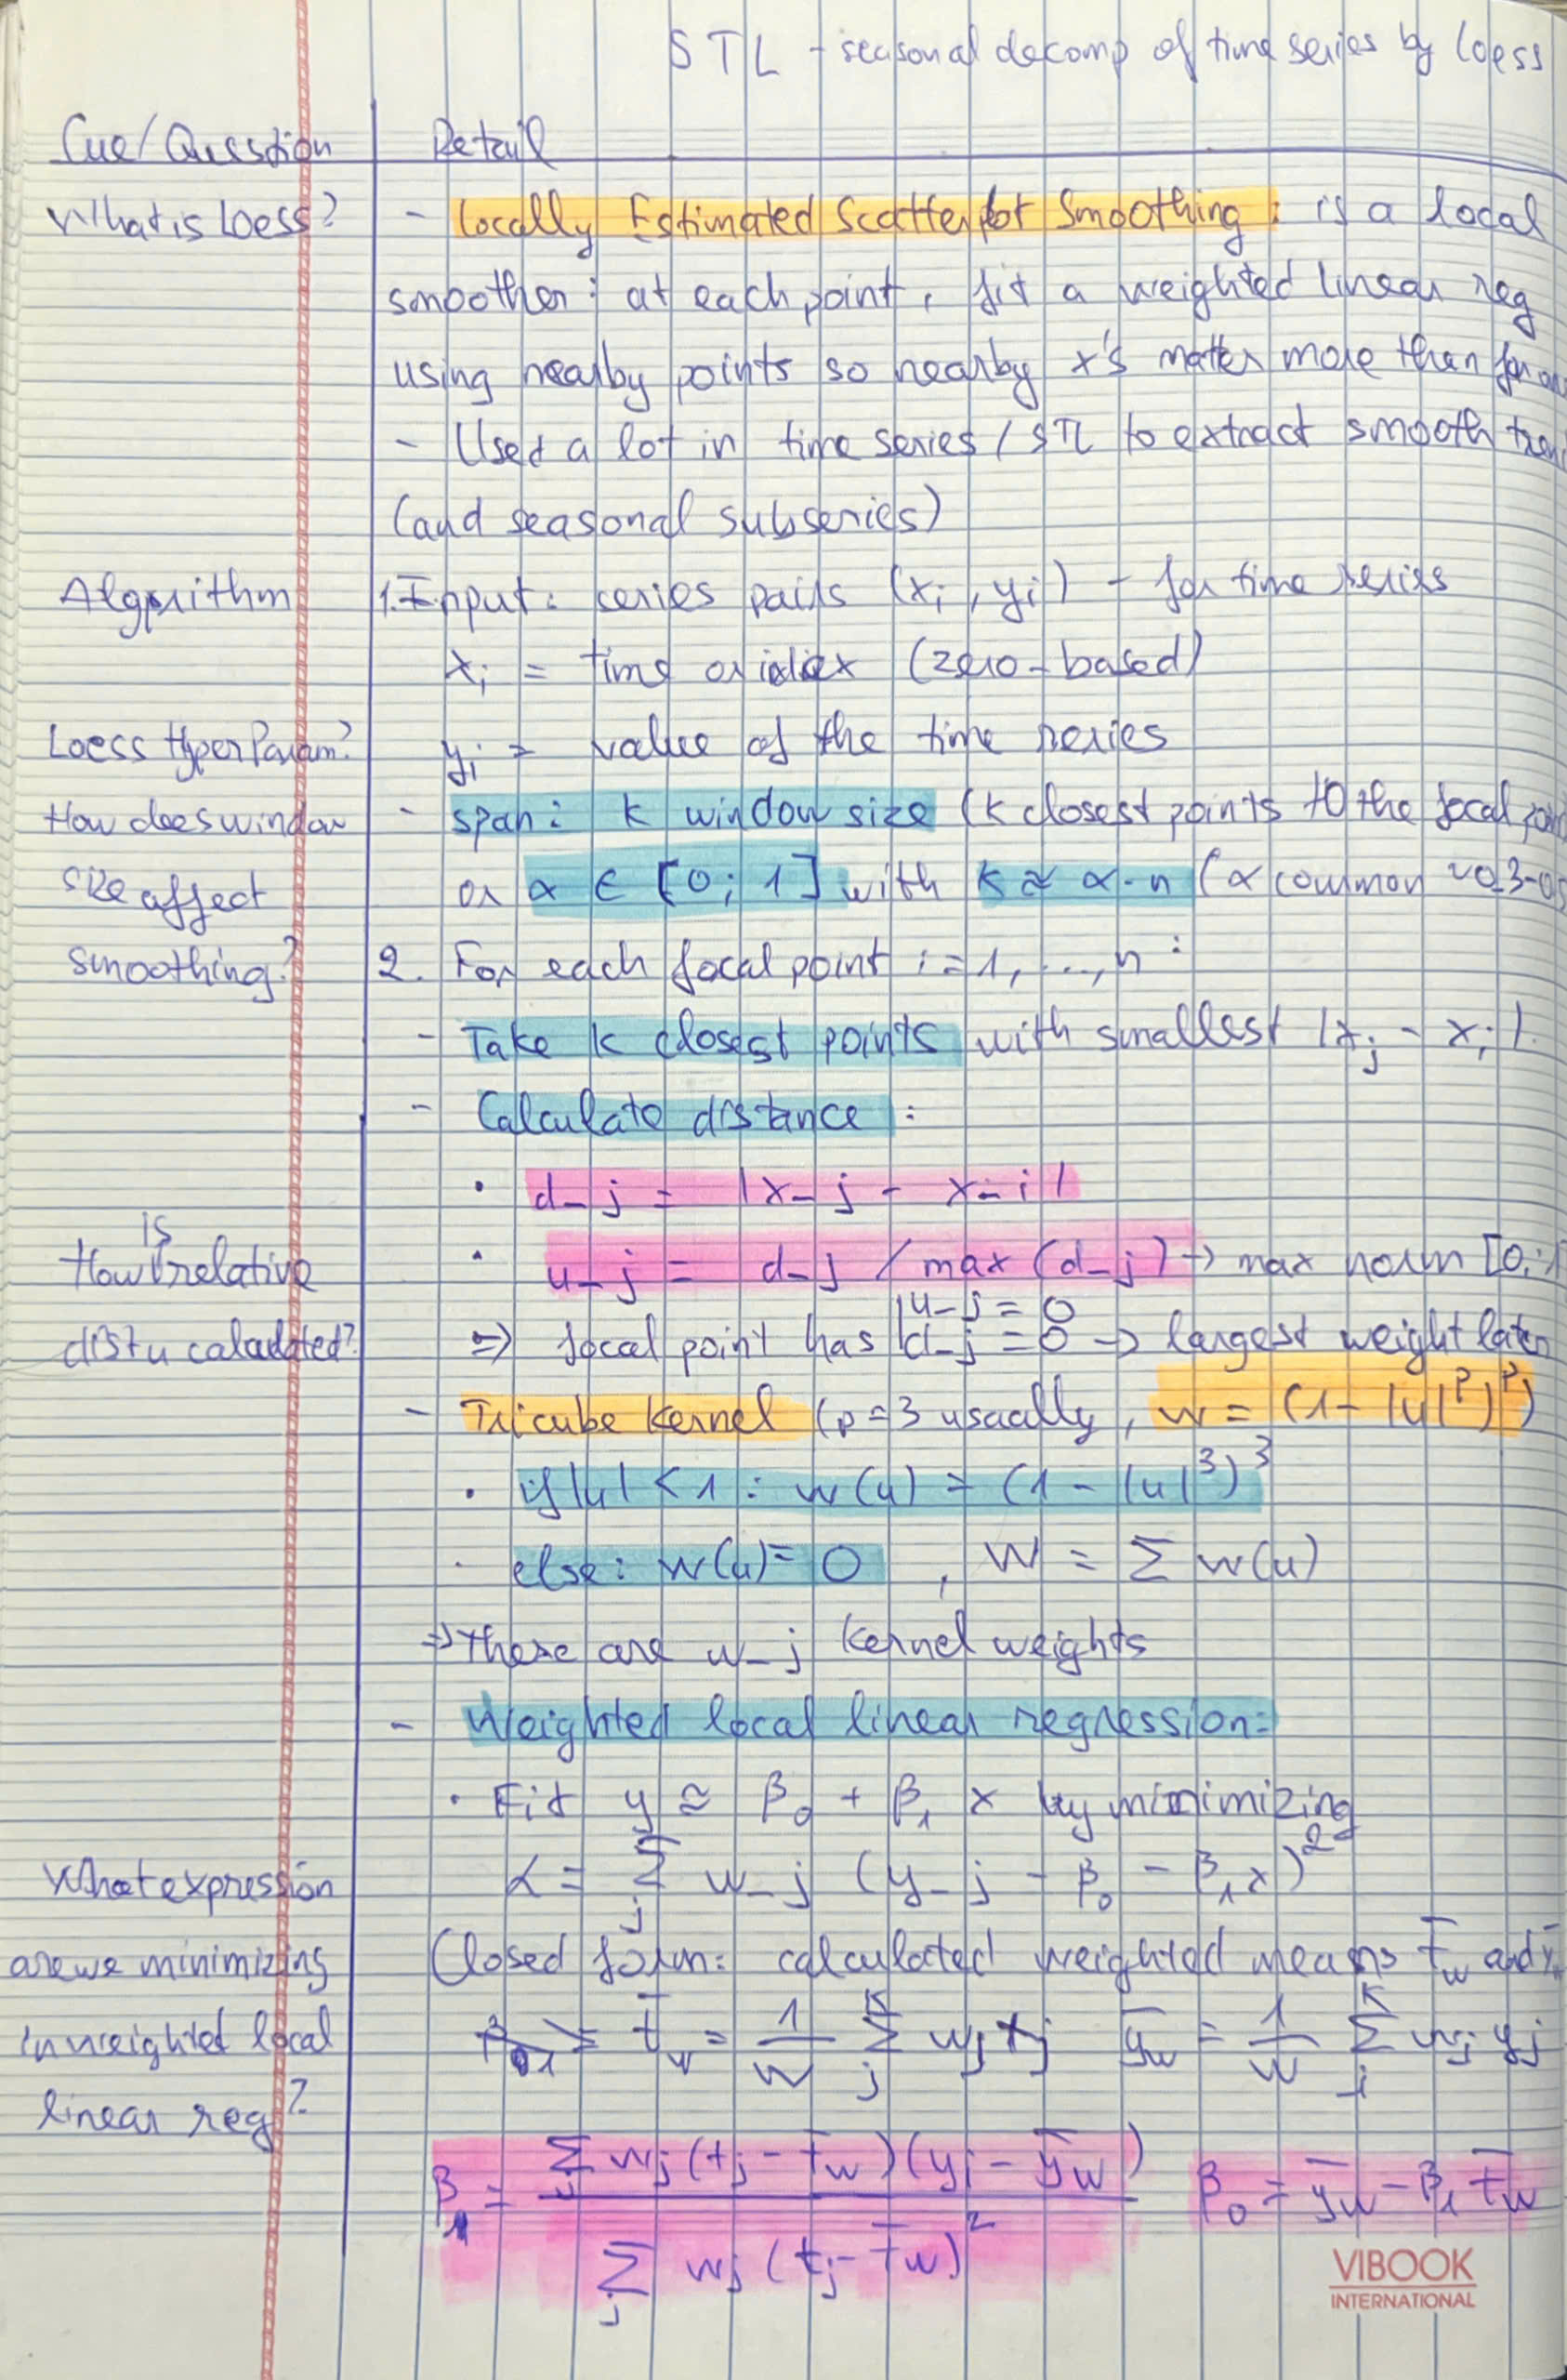
\includegraphics[width=0.92\textwidth,height=0.85\textheight,keepaspectratio]{Figures/Loess.jpg}
  \caption{Scan tay --- Loess (tương ứng Bảng~\ref{tab:cornell-loess}).}
  \label{fig:scan-loess}
\end{figure}

\begin{figure}[H]
  \centering
  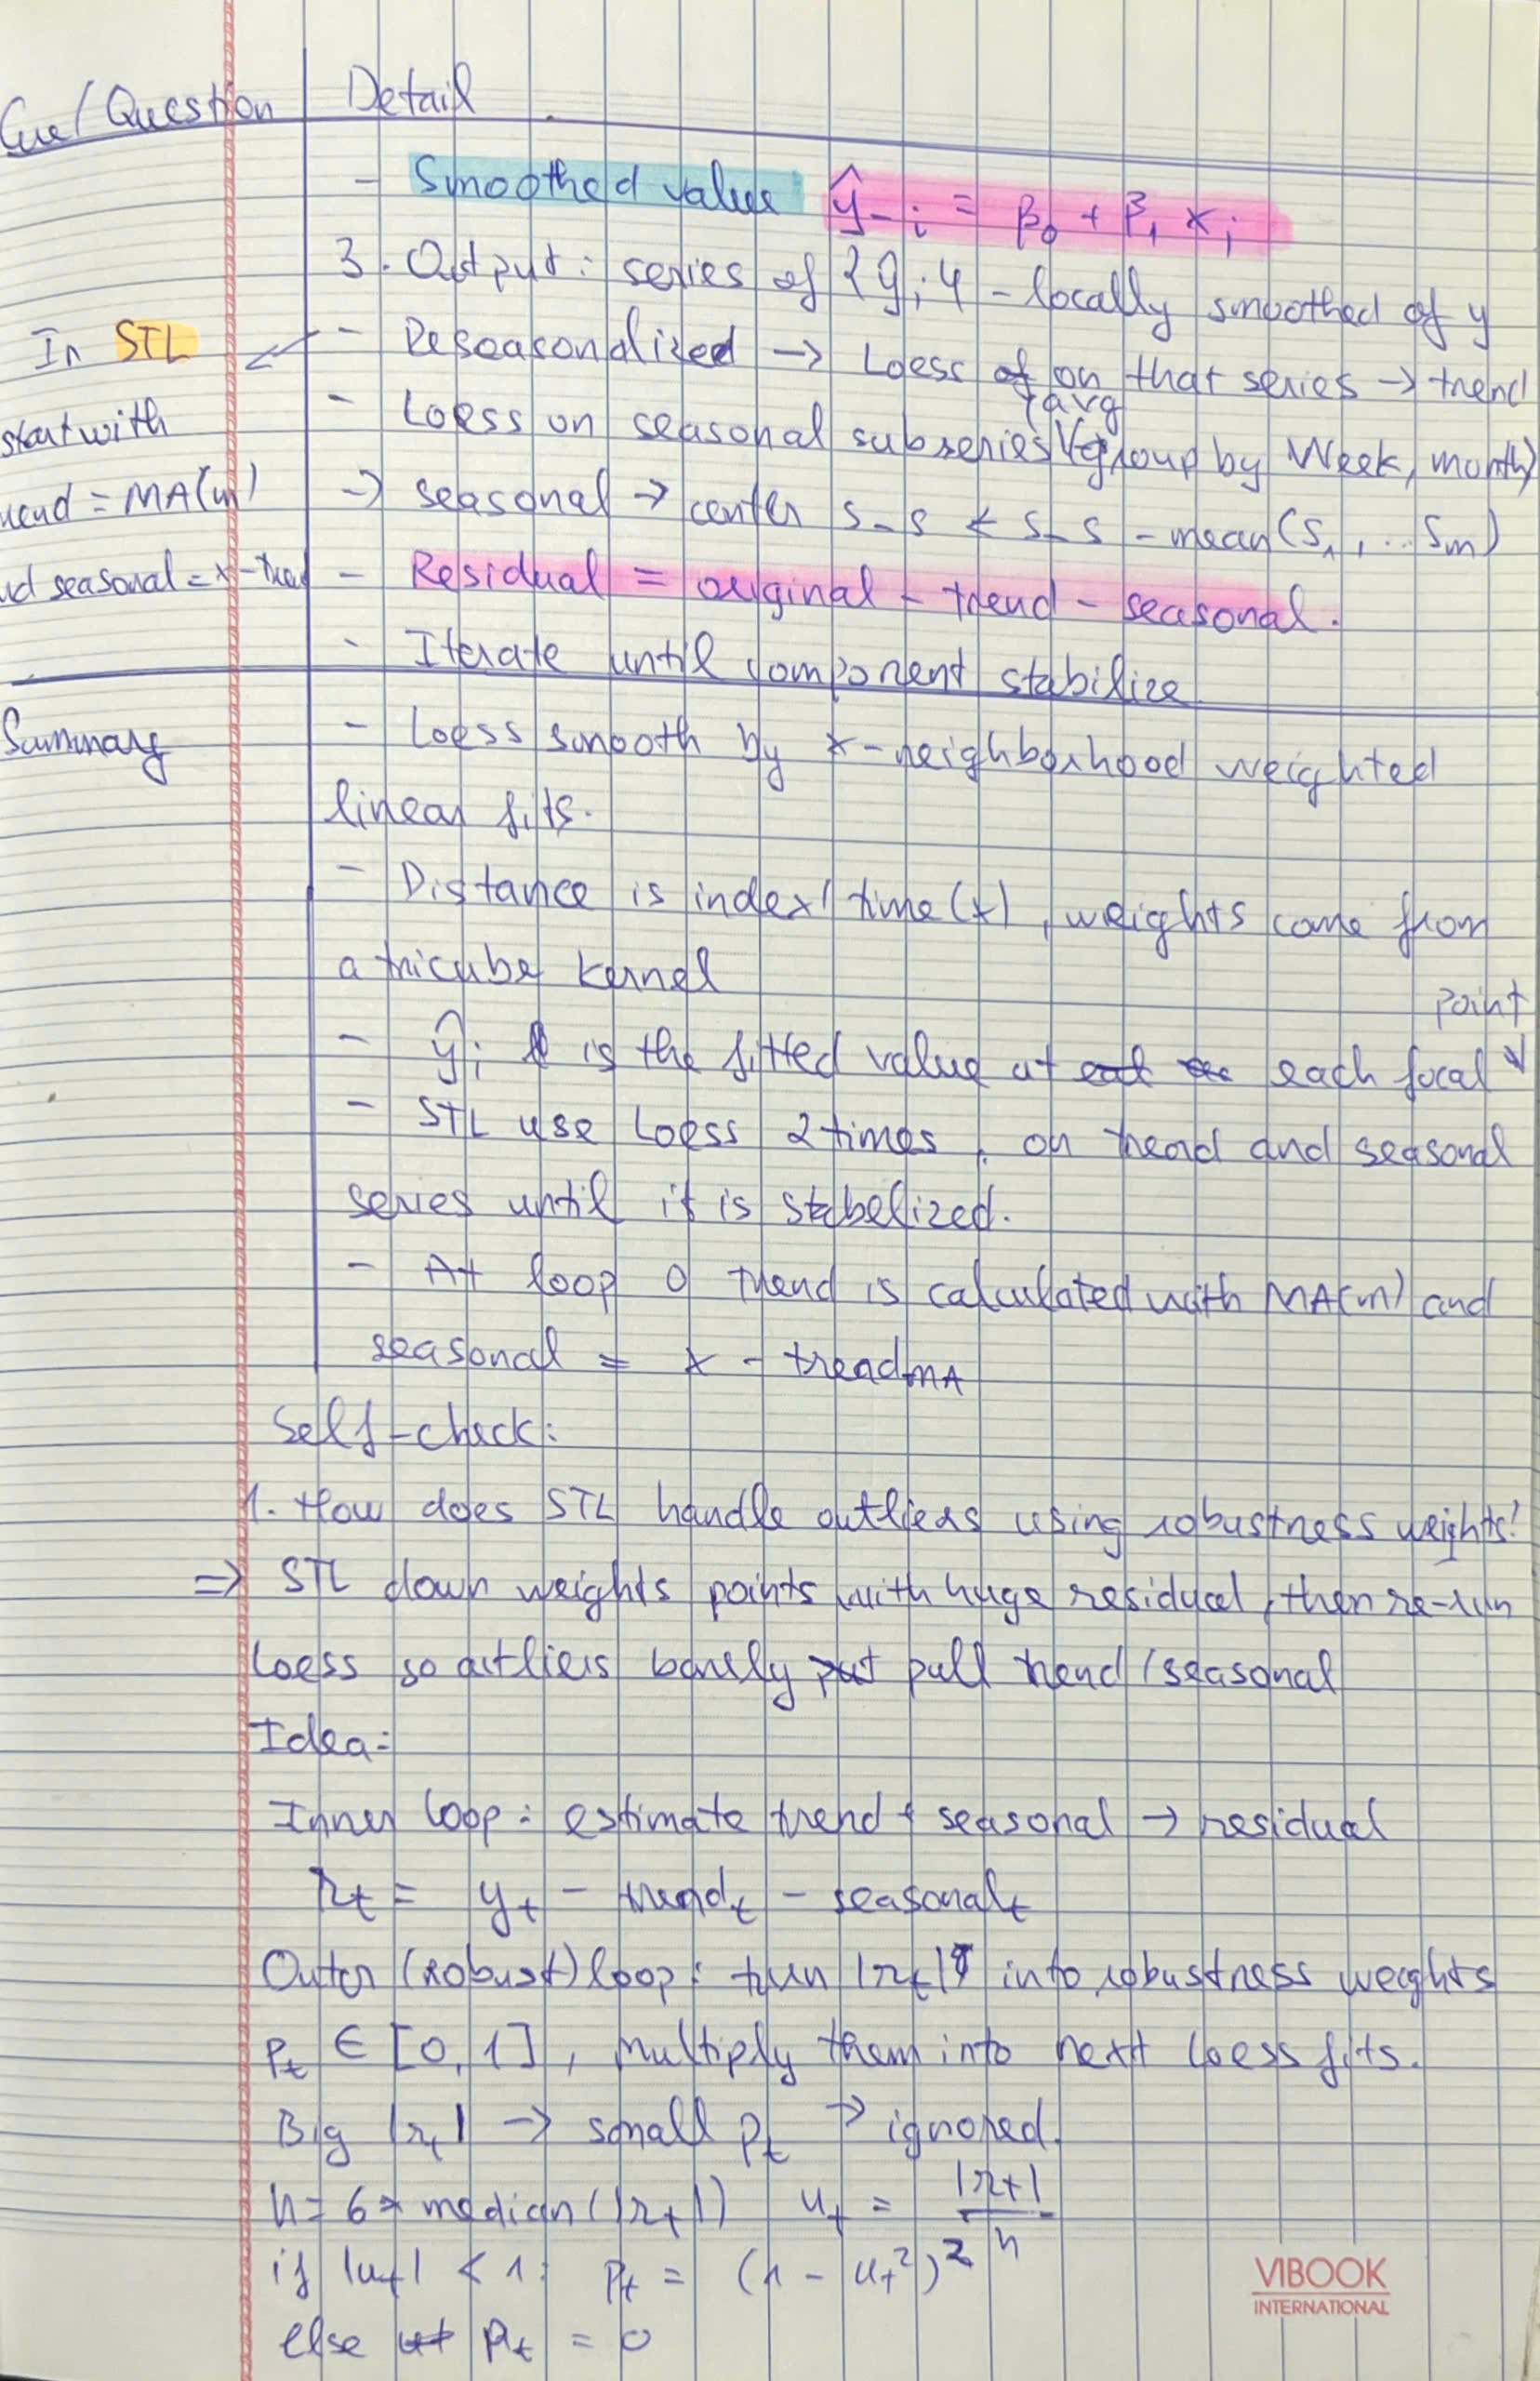
\includegraphics[width=0.92\textwidth,height=0.85\textheight,keepaspectratio]{Figures/STL.jpg}
  \caption{Scan tay --- STL + robustness (tương ứng Bảng~\ref{tab:cornell-stl},~\ref{tab:cornell-robust}).}
  \label{fig:scan-stl}
\end{figure}

\end{document}
